\section{Dataset Composition and Comparison}
This appendix provides a detailed view of the \MixtureVitae{} corpus, both in relation to other datasets and in its internal construction.
% \begin{table*}[t]
% \centering
% \renewcommand{\arraystretch}{1.5} % Adds a bit of vertical padding for readability
% \begin{tabular}{@{}l l l l l@{}}
% \toprule
% \textbf{Dataset} & \textbf{\makecell[l]{Size \\ (Tokens)}} & \textbf{\makecell[l]{Primary \\ Data Types}} & \textbf{\makecell[l]{Licensing \\ Philosophy}} & \textbf{\makecell[l]{Synthetic Data \\ Policy}} \\
% \midrule
% \textbf{Mixture Vitae} & \textbf{$\approx 300B$} & \textbf{\makecell[l]{Web, Curated, \\ Books, Synthetic}} & \textbf{\makecell[l]{Strictly Permissive \\ + Risk-Mitigated}} & \textbf{\makecell[l]{Included}} \\

% \makecell[l]{Common Corpus \\ \citep{commoncorpus2023}} & $\approx2T$ & \makecell[l]{Books, Science, \\ Legal, Web} & \makecell[l]{Strictly Permissive; \\ Provenance-focused} & Excluded \\

% \makecell[l]{The Common Pile \\ \citep{commonpile2023}} & $\approx 5T$ (est.) & \makecell[l]{Web, Books, Code, \\ Academic} & \makecell[l]{Strictly Permissive \\ (OKD)} & Excluded \\

% \makecell[l]{Dolma \\ \citep{soldaini2024dolma}} & $\approx 3T$ & \makecell[l]{Web, Academic, Code, \\ Books} & \makecell[l]{Permissive (ODC-BY); \\ Open Tooling} & Excluded \\

% \makecell[l]{KL3M Data Project \\ \citep{kl3m2024}} & $>2.5T$ & \makecell[l]{Legal, Financial, \\ Government} & \makecell[l]{Proprietary; Certified \\ "Fairly Trained"} & Excluded \\

% \makecell[l]{The Stack \\ \citep{kocetkov2022stack}} & $\approx 2.2T$ (est.) & Source Code & Strictly Permissive & Excluded \\
% \bottomrule
% \end{tabular}
% \caption{Comparison of large-scale pretraining datasets. Mixture Vitae is unique in its combination of a risk-mitigated licensing philosophy and the inclusion of synthetic data to enhance pretraining performance.\cmt[VM]{Which other datasets to include?}}
% \label{tab:dataset_comparison}
% \end{table*}


\begin{table*}[htbp]
\center
\caption{Comparison of large-scale pretraining datasets, grouped by their licensing philosophy to provide context for our performance results. \MixtureVitae{} is unique in its combination of a risk-mitigated licensing approach and the inclusion of a large subset of reasoning, coding and instruction synthetic data.} 
\label{tab:dataset_comparison}
\footnotesize
\renewcommand{\arraystretch}{1.5} % Adds vertical padding
\scalebox{0.88}{
\begin{tabular}{@{}l l l l@{}}
\toprule
\textbf{Dataset} & \textbf{\makecell[l]{Size \\ (Tokens)}} & \textbf{\makecell[l]{Primary \\ Data Types}} & \textbf{\makecell[l]{Licensing \\ Philosophy}} \\
\midrule
\multicolumn{4}{@{}l}{\textit{Non-Permissive / Mixed-License Baselines}} \\
\quad Nemotron-CC-HQ \citep{su2025nemotroncc} & $\approx$ 1.1T & Web, Synthetic & Unspecified \\
\quad DCLM-baseline \citep{li2024datacomplm} & $\approx$ 3.8T & Web, Code, Academic & Mixed / Unspecified \\
\quad FineWeb-Edu \citep{penedo2024} & $\approx$ 1.3T & Web (Educational) & Unspecified \\
\quad The Pile \citep{gao2020pile} & $\approx$ 183.28B & Web, Books, Code & Mixed / Unspecified \\
\quad SlimPajama \citep{shen2024slimpajamadcunderstandingdatacombinations} & $\approx$ 627B & Web, Books, Code & Mixed / Unspecified \\
\quad C4 \citep{raffel2020exploring} & $\approx$ 156B & Web & ODC-BY \\
\quad HPLT-2.0 (eng.) \citep{burchell2025} & $\approx$ 2.86T & Web, Books, News & Mixed / Unspecified \\
\midrule
\multicolumn{4}{@{}l}{\textit{Permissive Baselines}} \\
\quad CommonCorpus \citep{langlais2025commoncorpuslargestcollection} & $\approx$ 2T & Web, Curated & Strictly Permissive \\
\quad Comma-0.1 \citep{kandpal2025commonpilev018tb} & $\approx$ 1T & Web, Curated & Strictly Permissive \\
\quad KL3M \citep{bommarito2025kl3mdataprojectcopyrightclean} & $\approx$ 580B & Web, Curated & Strictly Permissive \\
\quad OLC \citep{min2024silo} & $\approx$ 228B & Web, Curated & Strictly Permissive \\
\midrule
\multicolumn{4}{@{}l}{\textit{Our Contribution}} \\
\quad \MixtureVitae{} & \textbf{$\approx$ \DatasetSize{}B} & \textbf{\makecell[l]{Web, Curated, \\  Synthetic}} & \textbf{\makecell[l]{Permissive-First, \\ Risk-Mitigated}} \\
\bottomrule
\end{tabular}
}

\end{table*}

\paragraph{Shard Definitions and Mixing.}
It is important to note that the dataset shards and categories listed in this appendix serve as logical groupings for transparency, licensing audits, and ablation analysis. They do not dictate a rigid sequential training order. As noted in the main text, the physical construction of training batches utilizes domain-aware packing to maximize local coherence, prioritizing the density of reasoning and factual tokens over these high-level taxonomic boundaries.

Table~\ref{tab:dataset_comparison} presents a high-level comparison of \MixtureVitae{} against the other prominent pretraining datasets evaluated in our experiments, detailing their respective sizes, primary data types, and licensing philosophies.

\begin{figure}[htbp] 
    \centering    
    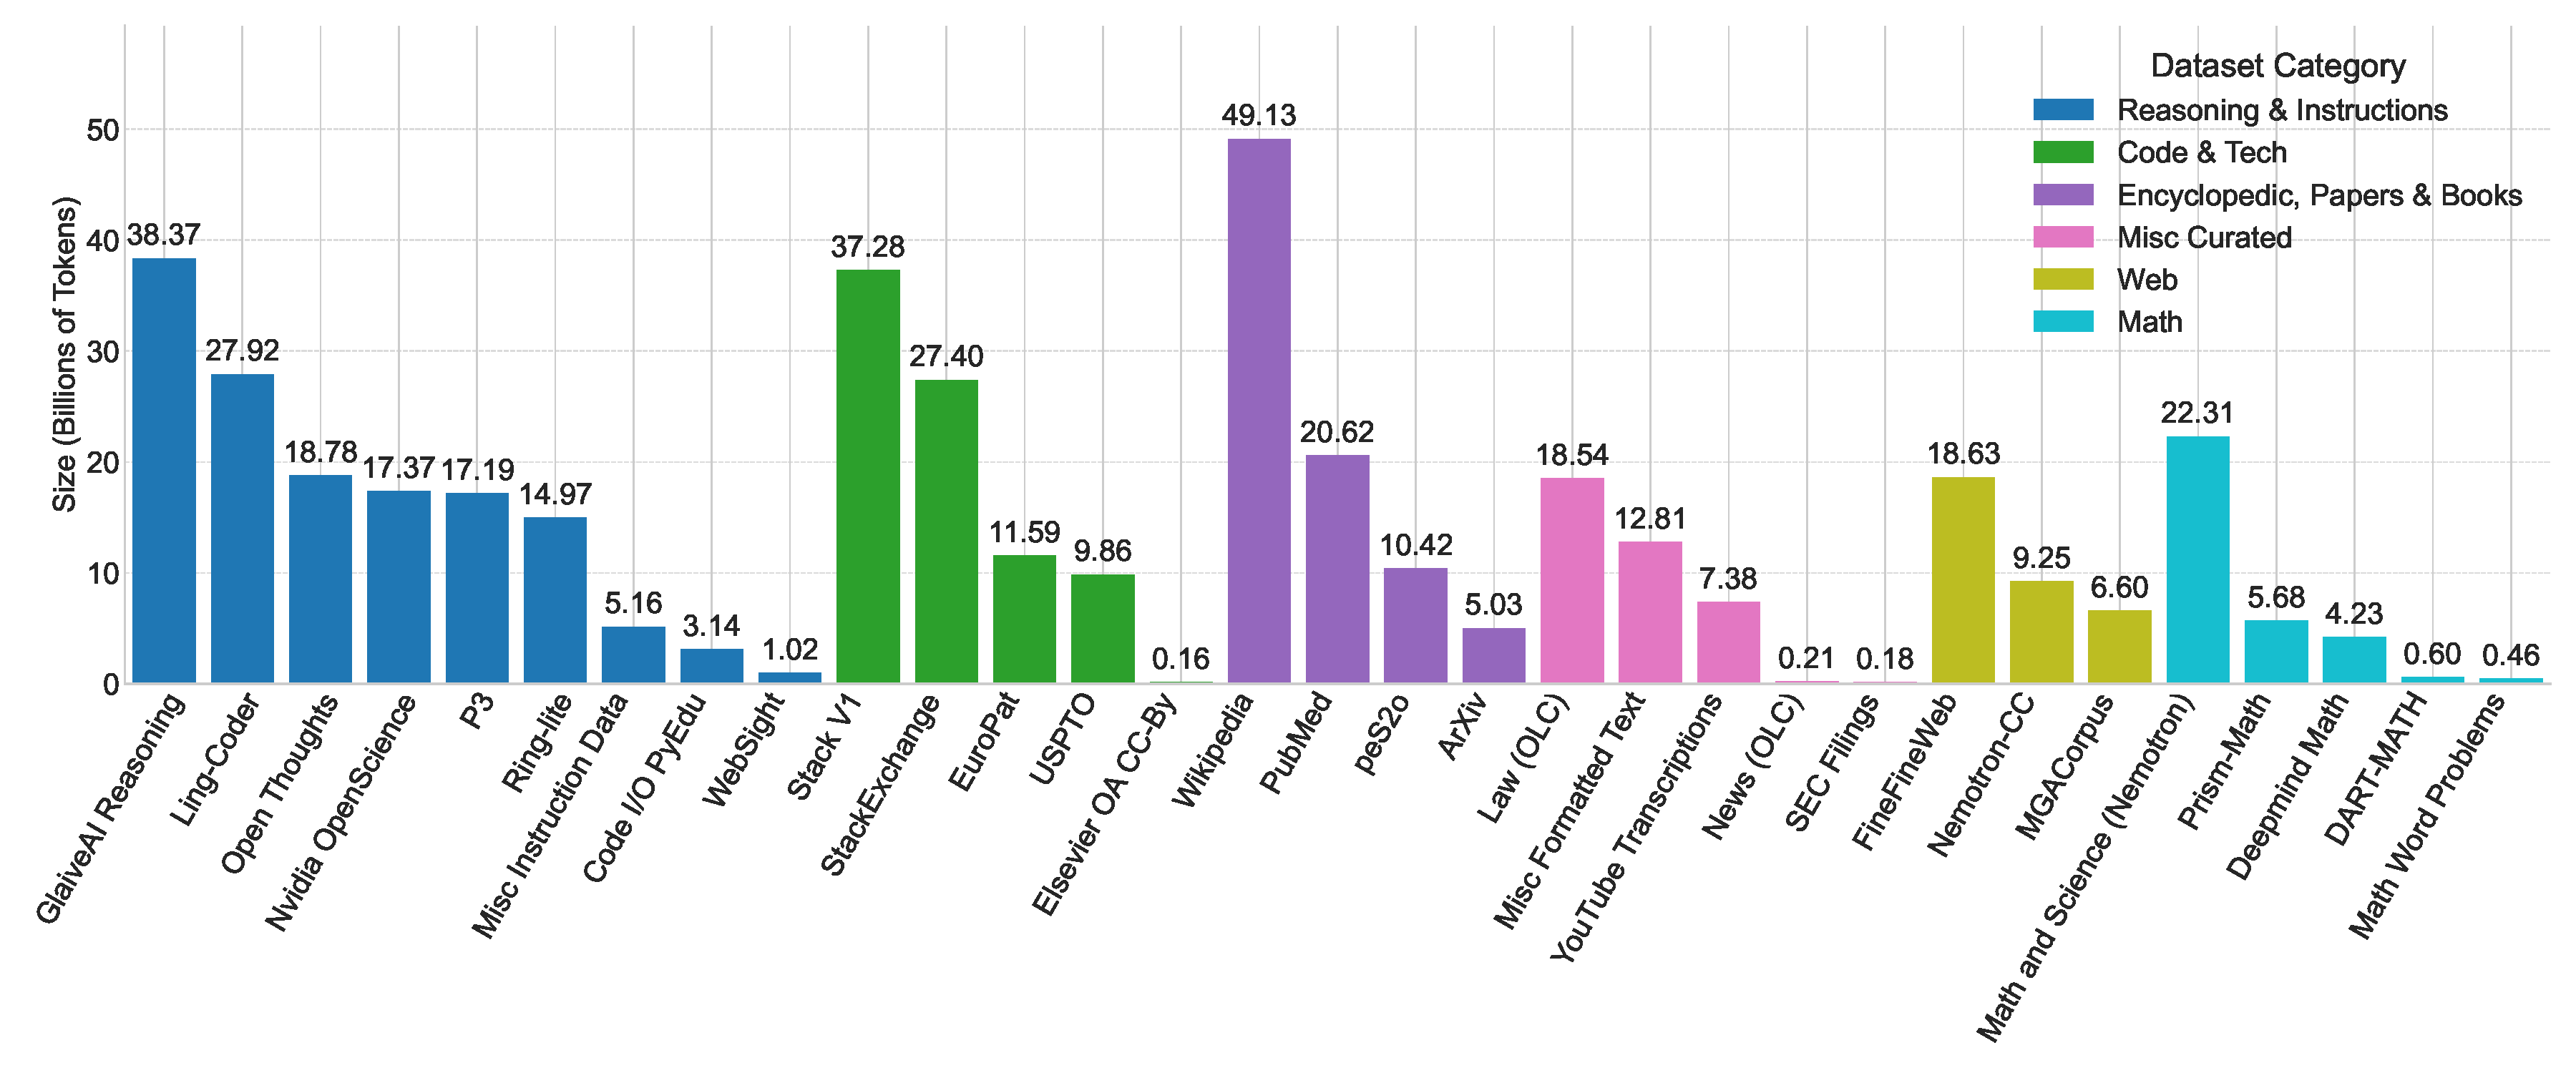
\includegraphics[width=1\linewidth]{figures/mixture_vitae_component_barchart.pdf}
      \caption[Detailed Composition of the MixtureVitae Dataset]{Detailed composition of the \MixtureVitae{} dataset.} 
    \label{fig:data_comp_deets}
\end{figure}

Figure~\ref{fig:data_comp_deets} presents the detailed composition of the \MixtureVitae{} dataset. The individual components are color-coded by their primary dataset category, as presented in the main text.

\begin{itemize}
    \item \textbf{Code \& Tech (Blue):} This domain is anchored by our largest code sources, Stack V1 and Ling-Coder, and supplemented by StackExchange.
    
    \item \textbf{Reasoning \& Instruction (Green):} The largest contributor to this category is Open Thoughts , followed by P3 and NVIDIA OpenScience.
    
    \item \textbf{Encyclopedic, Papers \& Books (Purple):} This category is dominated by Wikipedia, the single largest component in the dataset. It is complemented by large-scale text from PubMed  and arXiv.
    
    \item \textbf{Math (Cyan):} The math component is a diverse mixture of sources, led by the Math and Science (Nemotron) corpus and Prism-Math.
    
    \item \textbf{Web (Yellow):} Our web data is primarily sourced from corpora such as SEC Filings, MGACorpus, and FineFineWeb.
    
    \item \textbf{Misc Curated (Pink):} This category includes a variety of high-quality curated sources, notably Law (Open License Corpus) and YouTube Transcriptions.
\end{itemize}


% % This code is compatible with your existing packages.
% Assumes you have already loaded: booktabs, longtable, hyperref
% \refstepcounter{table}
\begin{longtable}{p{4cm} p{7cm} r}

% This is the caption that will appear above the table.
% \caption{Breakdown of the Dataset by Source and License}
% \label{tab:breakdown_by_license_type}\\

% --- HEADERS ---
% This header appears on the FIRST page of the table.
\toprule
\textbf{License Type} & \textbf{Source / Data} & \textbf{Size} \\
\midrule
\endfirsthead

% This header appears on ALL SUBSEQUENT pages of the table.
\multicolumn{3}{c}%
{{\bfseries\tablename\ \thetable{} -- continued from previous page}} \\
\toprule
\textbf{License Type} & \textbf{Source / Data} & \textbf{Size} \\
\midrule
\endhead

% --- FOOTERS ---
% This footer appears at the bottom of every page EXCEPT the last one.
\bottomrule
\multicolumn{3}{r}{{Continued on next page}} \\
\endfoot

% This footer appears only on the LAST page of the table.
\bottomrule

\endlastfoot

% --- WEB SECTION ---
\multicolumn{3}{c}{\large\textbf{Web}} \\
\multicolumn{3}{l}{\footnotesize\textit{*All data in this section subject to Common Crawl Terms of Uses}} \\
\midrule
Public Domain (copyright expired) & US Federal governmental websites including a small portion of Project Gutenberg out of copyright literature inclded in the web portion, & 6B \\
\addlinespace % Adds a little vertical space for readability
Risk-mitigated government data & Non US federal government works & 11B \\
\addlinespace
CC-BY-SA* licenses or more permissive & Specific curated websites and heuristicly mathced websites (See Sec. J) & 2B \\
\midrule

% --- CURATED SECTION ---
\multicolumn{3}{c}{\large\textbf{Curated}} \\
\midrule
Public Domain & US Case law, SEC 10K, Europat, USPTO & 4 B \\
\addlinespace
CC-BY-SA* licenses or more permissive & News, wiki,  Youtube, peS2o, Pubmed, Arxiv, Stackexchange, elsevier-oa-cc-by,  & 24.67+10.31+5.21+3.69B \\
\addlinespace
Non-GPL open source license (e.g., Open-RAIL, Apache, MIT) & Stackv1 and its derivatives & 6.4+18.64 B \\
\midrule

% --- INSTRUCT SECTION ---
\multicolumn{3}{c}{\large\textbf{Instruct}} \\
\midrule
CC-BY.* licenses or more permissive & math\_word\_problems & 1.2 GB \\
& Nemo\_science\_math & 79 GB \\
\addlinespace
Non-GPL open source license (e.g., Apache, MIT) & Prism\_math (cc-by-4.0), Os-q2, Formatted\_text (only websights), misc\_instruct (cc-by-4.0) & 105 GB \\
& Glaiveai-reasoning (apache), Ring-lite (apache), Open\_thoughts (apache), Ling-coder (apache), Few-shot (from \href{https://huggingface.co/datasets/Muennighoff/P3}{P3}, apache), misc\_instruct (apache 2.0), Math (apache 2.0) & 458.6 GB \\
& dart-math, misc\_instruct (MIT) & 5 GB \\
& pyedu\_reasoning & 11 GB \\
% \captionof{table}{Breakdown of the Dataset by Source and License}
\end{longtable}
\addtocounter{table}{-1} % Corrects the counter for the caption command
\begin{center}
    \captionof{table}{Breakdown of the Dataset by Source and License}
    \label{tab:breakdown_by_license_type}
\end{center}
